\section*{1.}

\subsubsection*{a)}

The most noticeable difference between the quality check applied
(\Cref{fig:qa_xco2}) and no quality check (\Cref{fig:no_qa_xco2})
is the smaller standard deviation within each latitude bin. Around half of the
data points is discarded by the quality check. The latitudinal variation in
\ch{XCO2} is more apparent in when the quality check is applied, removing the
unrealistic values of \ch{XCO2}. The reason why the quality discarded so many
data points, I would guess is mostly due to clouds interfering with the signal,
but at the high latitudes points might also been removed due to ice and snow
cover on the ground. By looking at MODIS Aqua true color images from NASA
worldview, there seem to be a lot of clouds between 30 - 40\degree N, which could
be the reason why the around half of the data points in that bin was discarded.   
\begin{figure}[htbp]
    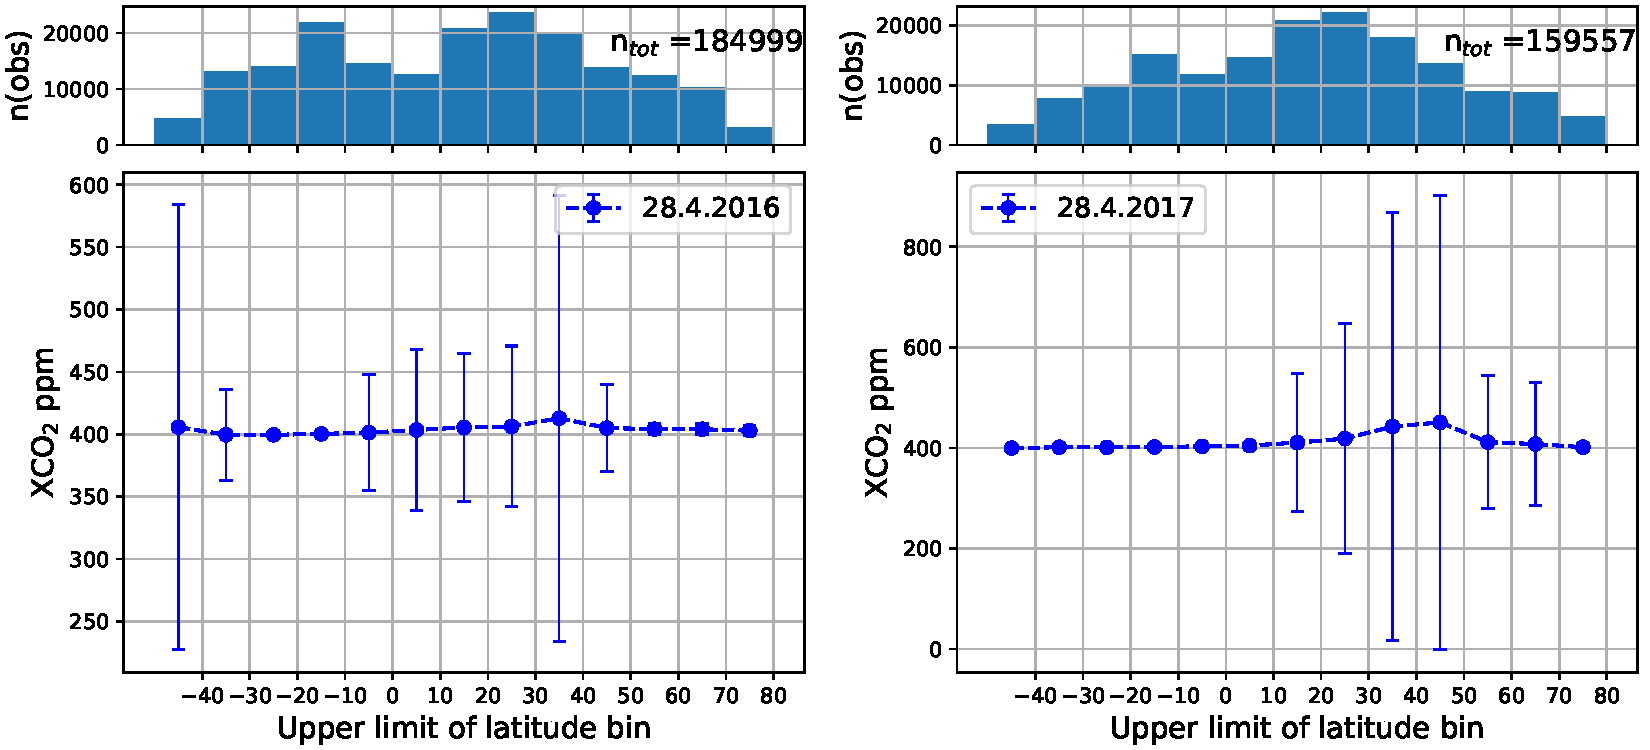
\includegraphics[width=\textwidth]{../xCO2.pdf}
    \caption{Bias corrected \ch{XCO2} from the OCO2 satellite from 28.04.2016 (left) 
    and 28.04.2017 (right), without quality flags applied. The upper panels 
    show the number of data points in each bin. The lower panels shows the \ch{XCO2} 
    concentration in ppm on the y-axis, along the x-axis is the upper limit of
    the latitude bins. The error bar represent $\pm$ one standard deviation.}
    \label{fig:no_qa_xco2}

\end{figure}

\begin{figure}[htbp]
    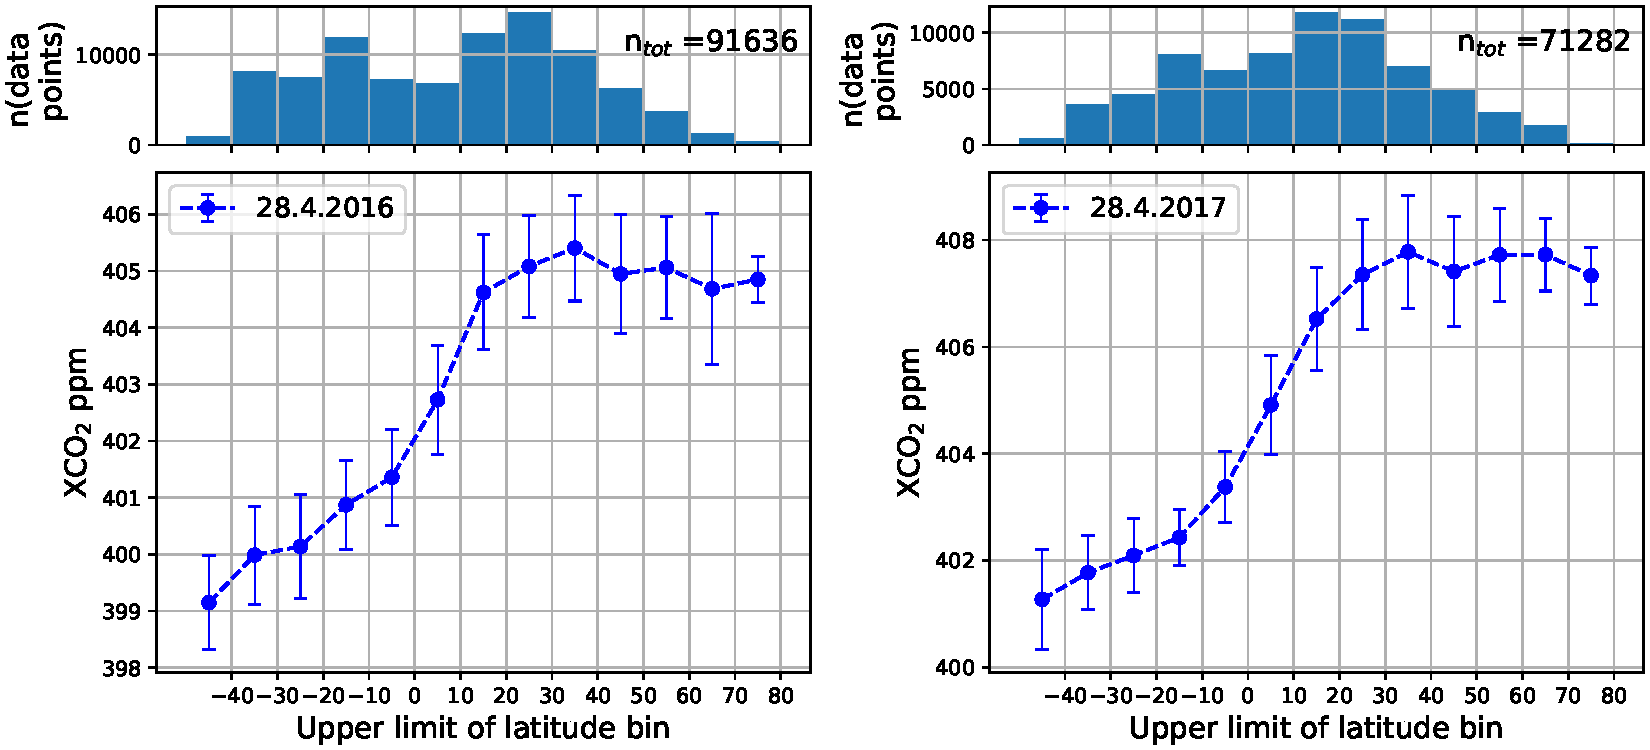
\includegraphics[width=\textwidth]{../qa_xCO2.pdf}
    \caption{Bias corrected XCO2 from the OCO2 satellite from 28.04.2016 (left) 
    and 28.04.2017 (right), with quality flags applied. The upper panels 
    show the number of data points in each bin. The lower panels shows the \ch{XCO2} 
    concentration in ppm on the y-axis, along the x-axis is the upper limit of
    the latitude bins. The error bar represent $\pm$ one standard deviation.}
    \label{fig:qa_xco2}

\end{figure}


